\section{Results and Evaluation}

\subsection{Prediction quality of the five methods}

\begin{table}[!htb]
\centering\small
\caption{Prediction quality (equal-site means over registered observation states). $^{\dagger}$Primary model,
selected on development log-MAE. Bold marks the best of the five main methods per column; CNP's 0\% FPR is
not bolded because it never predicts a low cell. Recall excludes Wellington Airport, which has no low cells.}
\label{tab:prediction}
% generated by report/make_tables.py -- do not edit by hand
\begin{tabular}{@{}lrrrrrrr@{}}
\toprule
 & \multicolumn{2}{c}{Development (4 sites)} & \multicolumn{5}{c}{Evaluation (4 sites)}\\
\cmidrule(lr){2-3}\cmidrule(l){4-8}
Method & log-MAE & Thick.\ (m) & log-MAE & Thick.\ (m) & Recall (\%) & FPR (\%) & F1\\
\midrule
GP & 0.658 & 0.614 & 0.509 & \textbf{0.400} & 14.0 & \textbf{1.9} & 0.11\\
XGBoost residual & 0.597 & 0.571 & 0.512 & 0.485 & 31.2 & 6.9 & 0.30\\
CNP & 0.833 & 0.774 & 0.657 & 0.430 & 0.0 & 0.0 & 0.00\\
TabPFN joint & 0.598 & \textbf{0.483} & \textbf{0.497} & 0.491 & 33.3 & 7.8 & 0.30\\
TabPFN + graph$^{\dagger}$ & \textbf{0.578} & 0.586 & 0.503 & 0.595 & \textbf{36.3} & 9.6 & \textbf{0.31}\\
\midrule
\multicolumn{8}{l}{\textit{TabPFN ablation (the fine-tuned joint row above completes the set)}}\\
\quad Residual, pretrained weights & 0.627 & 0.642 & 0.506 & 0.494 & 23.4 & 5.9 & 0.23\\
\quad Residual, fine-tuned weights & 0.598 & 0.626 & 0.502 & 0.509 & 22.4 & 6.0 & 0.22\\
\quad Residual, fine-tuned + sign guard & 0.598 & 0.573 & 0.503 & 0.497 & 32.1 & 7.3 & 0.30\\
\quad Joint, pretrained weights & 0.604 & 0.485 & 0.495 & 0.480 & 34.9 & 7.5 & 0.32\\
\bottomrule
\end{tabular}

\end{table}

\textbf{Main comparison.} TabPFN joint has the lowest evaluation profile error (\cref{tab:prediction}): 0.497,
2.9\% below XGBoost. TabPFN + graph is 1.8\% below XGBoost. The margins are small and site-dependent. Joint
beats XGBoost in 9 of 12 site--seed cells, by 0.9--3.9\% per site. At New Lock the GP is better than every
TabPFN hybrid (0.976 against 1.034). On evaluation sites the GP has the lowest thickness error (0.400\,m),
but mainly because it rarely predicts low cells: its recall is 14\%. On development sites its thickness
error is the second worst. The graph union buys the highest recall (36\%), at the cost of the highest FPR
(9.6\%) and the largest thickness error. CNP never predicts $\qc<1$\,MPa, a genuine negative result for a
median-trained set model on rare events.

\textbf{Site difficulty.} Site difficulty dominates model differences (\cref{fig:models}): log-MAE is
0.11--0.24 at Wellington Airport and 0.98--1.14 at New Lock.

\textbf{TabPFN ablation.} Source-site fine-tuning lowered the raw residual's development log-MAE from 0.627
to 0.598. On evaluation sites, however, the pretrained and fine-tuned joint models differ by under 0.002.
Most of the thickness gain comes from the spatial blend and the whole-profile decision (development 0.626
$\rightarrow$ 0.483\,m), not from the Transformer weights. The improvement belongs to the hybrid, not to
TabPFN alone.

\textbf{Error analysis.} In the full-plan predictions at New Lock, error peaks at 4--6\,m, where 23\% of cells are low.
In that band the primary model recovers 53\% of low cells but raises 85 false alarms. The GP flags only 1--3\%
of cells as low, against 9--23\% true, so it under-predicts soft layers throughout. Thin layers below the
0.25\,m grid add irreducible error.

\begin{figure}[!htb]
\centering
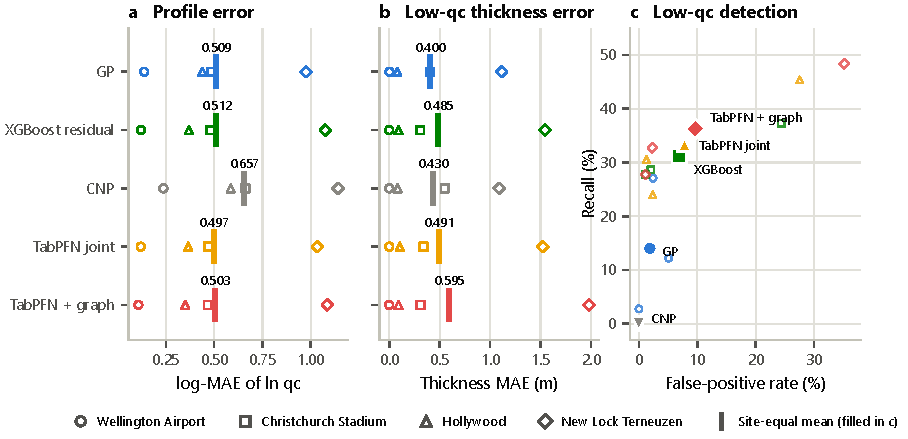
\includegraphics[width=\linewidth]{fig04_five_models.pdf}
\caption{Five AI methods on identical observation states at the four evaluation sites. Open marks are site
means (shape = site), and bars and filled circles are equal-site means. (c)~Low-cell recall against FPR;
recall is undefined at Wellington Airport.}
\label{fig:models}
\end{figure}

\subsection{Selection, stopping and audit}

\begin{figure}[!htb]
\centering
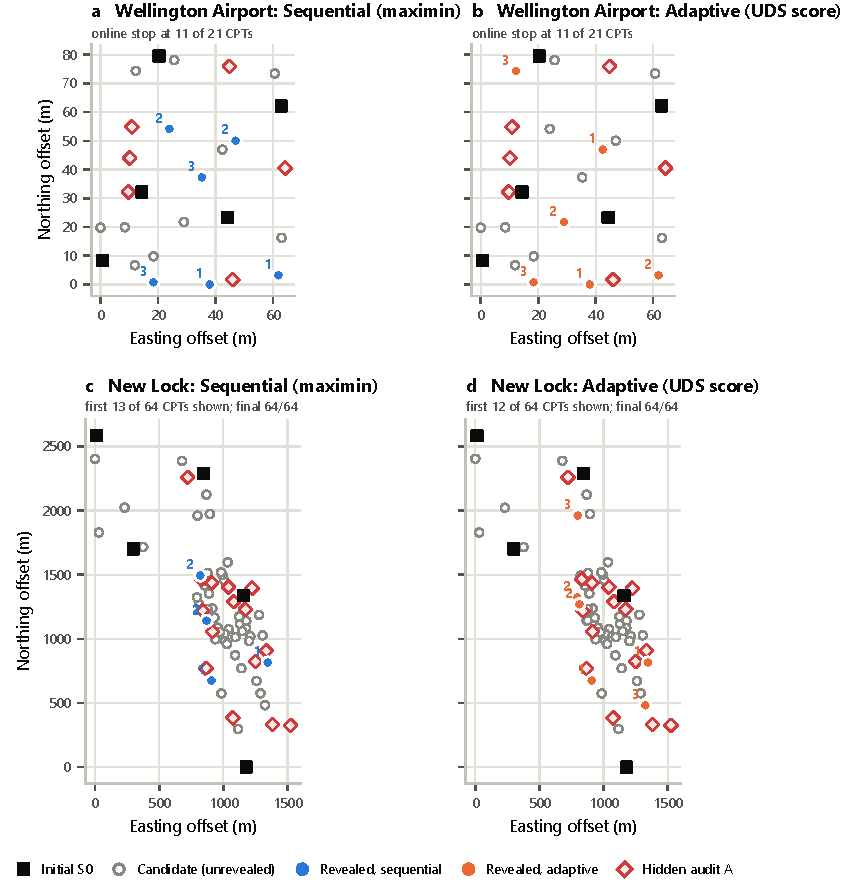
\includegraphics[width=0.62\linewidth]{fig03_selection_maps.pdf}
\caption{Selection maps, seed 17. (a,~b)~Wellington Airport at the online stop. (c,~d)~New Lock after the
first 12--13 CPTs. Numbers give the round in which a position was revealed. The adaptive score combines GP
uncertainty $U$, model disagreement $D$ and distance $d$.}
\label{fig:maps}
\end{figure}

\textbf{Where each policy samples.} The adaptive score does choose different locations from maximin
(\cref{fig:maps}). At New Lock it concentrates on the dense, variable central cluster where uncertainty and
disagreement are high, whereas maximin spreads out.

\textbf{Quality as CPTs are added (\cref{fig:quality}).} At the three easier sites audit quality is inside
the targets from the first few CPTs. At New Lock the error falls steeply over the first 15 CPTs and then
plateaus at log-MAE $\approx0.9$ and thickness MAE $\approx1.1$--1.5\,m, above both targets, even with all
64 CPTs.

\begin{table}[!htb]
\centering\small
\caption{Decision outcomes at the evaluation sites (means of three seeds). $|A|$ is the number of audit
positions. ``Full plan passes'' counts the seeds in which even the full plan meets the audit targets.
Oracle~$N$ is the smallest adaptive count that would have passed, found with hindsight; it is a
diagnostic, not a policy. Net is the owner's benefit of the adaptive policy at $\alpha=1$.}
\label{tab:decisions}
% generated by report/make_tables.py -- do not edit by hand
\begin{tabular}{@{}lrrrrrrrrr@{}}
\toprule
 & & & \multicolumn{2}{c}{CPTs at stop} & \multicolumn{2}{c}{Saving (\%)} & Full plan & Oracle & Net\\
\cmidrule(lr){4-5}\cmidrule(lr){6-7}
Site & $N_{\text{full}}$ & $|A|$ & Seq. & Adapt. & Seq. & Adapt. & passes & $N$ (adapt.) & k\euro\\
\midrule
Wellington Airport & 21 & 6 & 11.0 & 11.0 & 47.6 & 47.6 & 3/3 & 9 & +23.3\\
Christchurch Stadium & 18 & 5 & 18.0 & 18.0 & 0.0 & 0.0 & 3/3 & 9 & $-$12.6\\
Hollywood & 20 & 5 & 18.7 & 20.0 & 6.7 & 0.0 & 3/3 & 13--14 & $-$11.9\\
New Lock & 64 & 16 & 64.0 & 64.0 & 0.0 & 0.0 & 0/3 & none & $-$55.9\\
\midrule
Equal-site mean &  &  &  &  & 13.6 & 11.9 &  &  & $-$14.3\\
\bottomrule
\end{tabular}

\end{table}

\textbf{Stopping outcomes.} No early stop failed the audit (\cref{tab:decisions}, \cref{fig:outcomes}), but
the evidence is thin. Only 7 of the 24 evaluation trajectories stopped early: 6 at Wellington Airport,
where every audited state passes, and 1 at Hollywood (Sequential, seed~17). The rule's real value is that
it never stopped at New Lock, where every early stop would have failed. A naive rule that stops at the
ninth CPT would have made 7 false stops (all six New Lock runs plus one at Hollywood). Ablations show that
the leave-group-out support error carries this safety: without it the evaluation runs make 3 (Sequential)
and 2 (Adaptive) false stops, whereas dropping any other signal adds none.

\textbf{Savings.} Equal-site savings were 13.6\% (Sequential) and 11.9\% (Adaptive). Wellington Airport,
21\,$\rightarrow$\,11 CPTs (47.6\%), is the only adaptive saving, and Sequential saved exactly the same
there. Eleven CPTs is the earliest stop the rule allows, so this saving reflects how uniform the site is,
not fine-grained learning.

\textbf{Adaptive against Sequential.} Adaptive location choice showed no detectable advantage. Across all
24 site--seed pairs on the eight replay sites, the two policies' stopping counts differed only 3 times, and
in both directions. At matched CPT counts the sign of the audit-error difference varies across sites and
seeds.

\textbf{Low cells and audit size.} The low-cell targets (recall $\ge0.5$, FPR $\le0.1$) failed at all three
sites that contain low cells. Audit sets are small (5--6 positions, 16 at New Lock), which limits every
site-level verdict.

\begin{figure}[!htb]
\centering
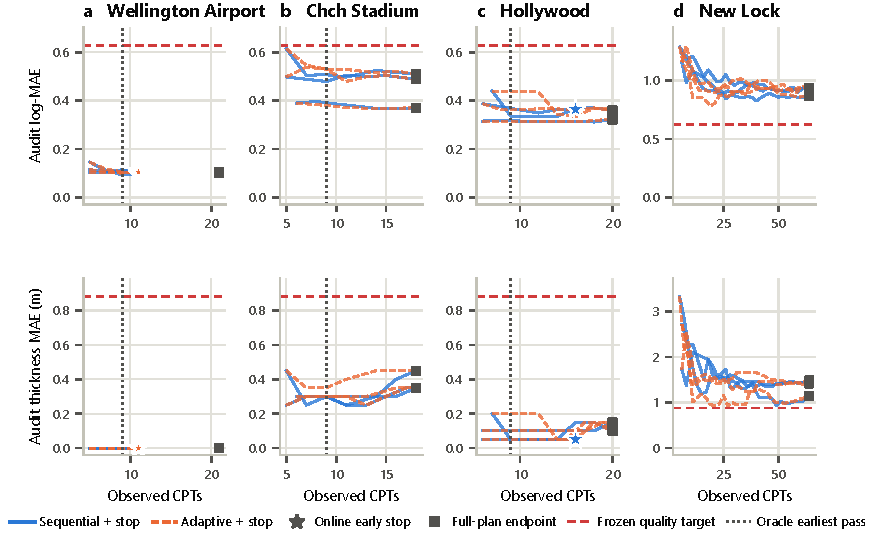
\includegraphics[width=\linewidth]{fig05_quality_vs_cpts.pdf}
\caption{Hidden-audit quality as CPTs are added (three seeds per policy). Stars mark online early stops,
squares the full plan, red dashed lines the frozen targets, and dotted lines the earliest passing count
found with hindsight (none at New Lock). Step changes reflect the small audit sets.}
\label{fig:quality}
\end{figure}

\begin{figure}[!htb]
\centering
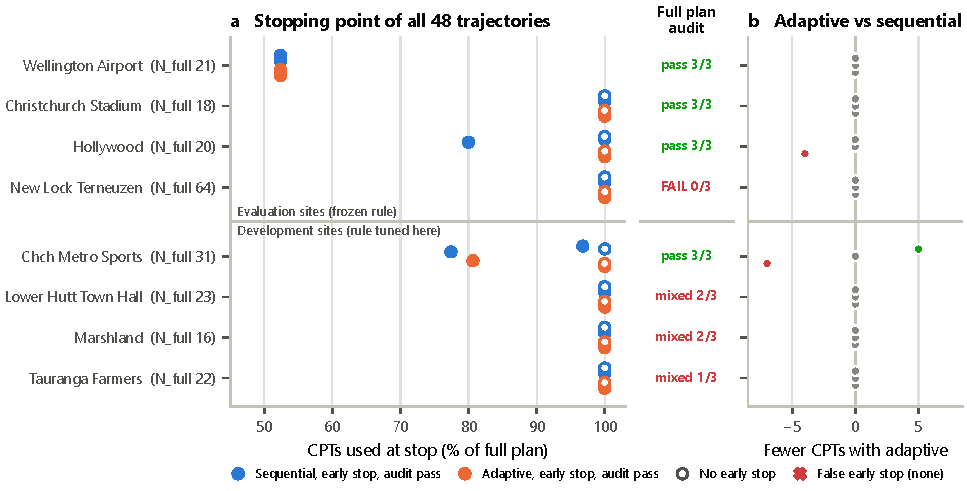
\includegraphics[width=\linewidth]{fig06_site_outcomes.pdf}
\caption{Stopping points of all 48 Sequential and Adaptive trajectories (8 sites $\times$ 3 seeds $\times$ 2
policies). (a)~CPTs used at the stop, with the full-plan audit verdict per site. (b)~CPTs saved by Adaptive
relative to Sequential, paired by seed.}
\label{fig:outcomes}
\end{figure}

\textbf{The rule is safe but conservative.} With hindsight, Christchurch Stadium already met the targets
with 9 of 18 CPTs, and Hollywood with 13--14 of 20 (Adaptive). Yet both Adaptive runs went to the full plan.
No single signal is to blame. At Christchurch Stadium, $\Delta Q_{90}$ and the GP uncertainty block the
most rounds; at Hollywood, $\Delta Q_{90}$ and $\Delta H_{90}$ block about equally often. $\Delta H_{90}\le0$ allows changes at up to 10\% of positions. Its
value of zero is a quantile tie in the development data, not a deliberately chosen tolerance. GP
uncertainty was only weakly related to actual audit error on evaluation sites (mean Spearman $\rho=0.21$,
against 0.60 on development sites).

\subsection{Economic value}

\textbf{Wellington Airport.} The observed counts were priced in the scenario (\cref{fig:econ}). The adaptive
policy yields $+$\eur{23,300}: (i)~\eur{7,500} from ten avoided CPTs; (ii)~\eur{10,250} of avoided project cost and \eur{6,150} of earlier-opening benefit, from finishing 2.05 days earlier; (iii)~less \eur{600} of AI cost.
Sequential stopping earns the same amount, so this benefit comes from staged stopping, not from AI location
choice.

\textbf{Other sites.} The other three sites are negative, from $-$\eur{11,900} to $-$\eur{55,900}, although
they used no extra CPTs. The staged campaign adds a 0.25-day decision delay at every batch transition. At
New Lock there are 27--29 transitions, which delay completion by 6.9 days. With zero delay these losses
shrink to the \eur{600} AI cost. With a one-day delay New Lock would lose \eur{222,000}, and Wellington
Airport would still gain \eur{5,300}. Across all four evaluation sites the mean is $-$\eur{14,300} for
Adaptive and $-$\eur{13,500} for Sequential.

\textbf{Sensitivity.} At $\alpha=0.5$ Wellington Airport falls to \eur{15,100}. No site changes sign within
any tested range.

\begin{figure}[!htb]
\centering
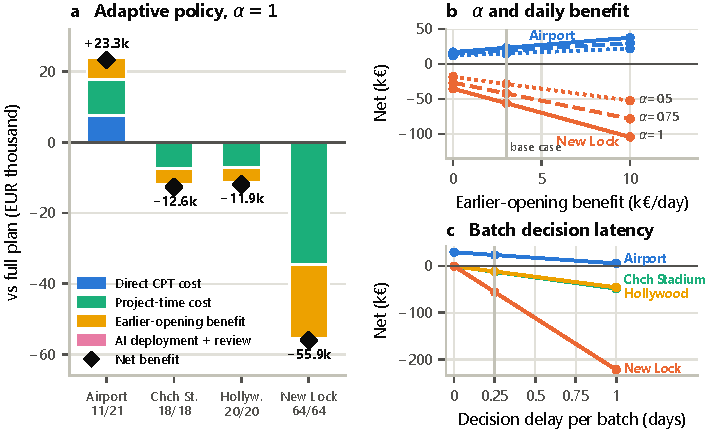
\includegraphics[width=\linewidth]{fig07_economics.pdf}
\caption{Owner's financial scenario, EUR 2025, Adaptive policy (mean of three seeds). (a)~Benefit components
relative to the full plan at $\alpha=1$. (b)~Net benefit as $\alpha$ and the daily earlier-opening benefit
vary (Wellington Airport and New Lock; the vertical line marks the base case). (c)~Net benefit against the
decision delay per batch.}
\label{fig:econ}
\end{figure}
